\section{Sp\-Copy\-To\-Texture3d\-Fb.h File Reference}
\label{SpCopyToTexture3dFb_8h}\index{SpCopyToTexture3dFb.h@{SpCopyToTexture3dFb.h}}
{\tt \#include \char`\"{}Sp\-Stream\-Feedback.h\char`\"{}}\par
{\tt \#include \char`\"{}Sp\-Gl\-Headers.h\char`\"{}}\par


Include dependency graph for Sp\-Copy\-To\-Texture3d\-Fb.h:\begin{figure}[H]
\begin{center}
\leavevmode
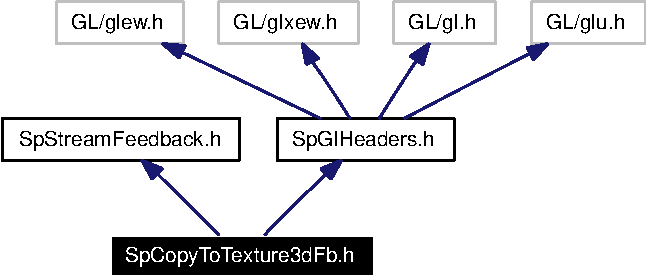
\includegraphics[width=172pt]{SpCopyToTexture3dFb_8h__incl}
\end{center}
\end{figure}
\subsection*{Namespaces}
\begin{CompactItemize}
\item 
namespace {\bf Spark}
\end{CompactItemize}
\subsection*{Classes}
\begin{CompactItemize}
\item 
class {\bf Spark::Sp\-Copy\-To\-Texture3d\-Fb}
\begin{CompactList}\small\item\em Sliced 3D Copy To Texture (CTT) feedback mechanism via Open\-GL. \item\end{CompactList}\end{CompactItemize}
